\documentclass[t,usenames,dvipsnames]{beamer}
\usetheme{Copenhagen}
\setbeamertemplate{headline}{} % remove toc from headers
\beamertemplatenavigationsymbolsempty

\usepackage{amsmath, tikz, xcolor, array, graphicx}
\usetikzlibrary{arrows.meta}

\title{Basic Set Theory and Interval Notation}
\author{}
\date{}

\AtBeginSection[]
{
  \begin{frame}
    \frametitle{Table of Contents}
    \tableofcontents[currentsection]
  \end{frame}
}

\begin{document}

\begin{frame}
    \titlepage
\end{frame}

\section{}

\begin{frame}{Sets}
A \alert{set} is a well-defined collection of things called \emph{elements}. By ``well-defined", we mean that we will know whether or not an element belongs in the set.
\end{frame}

\begin{frame}{Ways of Describing Sets}
	\begin{itemize}	
		\item Verbally  \newline\\  \pause
		\item Roster Method (list out everything)	\newline\\  \pause
		\item Set-Builder Method (give a rule to generate the items in the set)   \newline\\  \pause
		\begin{itemize}
		    \item $A = \left\lbrace  x \mid x \text{ is a positive even integer.} \right\rbrace = \{2, \, 4, \, 6, \, 8, \, \dots\}$
		\end{itemize}
	\end{itemize}   \vspace{11pt}  \pause
	
The \alert{empty set} is a set with no elements (symbol is $\varnothing$). This is notation used for ``No Solution" answers.
\end{frame}

\section{Write a set using interval notation}

\begin{frame}{Interval Notation}
\begin{center}
\setlength{\extrarowheight}{8pt}
\scalebox{0.9}{
\begin{tabular}{|c|c|c|}
\hline \textbf{Interval Notation} & \textbf{Set-Builder Notation} & \textbf{Graph} \\[5pt] 
\hline 
$(4, \, 9)$ & $\lbrace x \mid 4<x<9 \rbrace$ & 
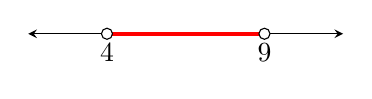
\begin{tikzpicture}[baseline=(current bounding box.north)]
    \coordinate (A) at (0,0);
    \coordinate (B) at (2,0);
    \draw [<->, >=stealth] (-1,0) -- (3,0);
    \node at (A) [anchor = north] {$4$};
    \node at (B) [anchor = north] {$9$};
    \draw [red, ultra thick] (A) -- (B);
    \draw [fill=white] (A) circle (2pt);
    \draw [fill=white] (B) circle (2pt);
\end{tikzpicture}
\\
\hline $[4, \, 9]$ & $\lbrace x \mid 4\leq x \leq 9 \rbrace$ & 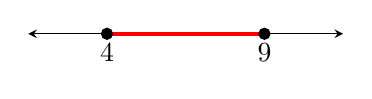
\begin{tikzpicture}[baseline=(current bounding box.north)]
    \coordinate (A) at (0,0);
    \coordinate (B) at (2,0);
    \draw [<->, >=stealth] (-1,0) -- (3,0);
    \node at (A) [anchor = north] {$4$};
    \node at (B) [anchor = north] {$9$};
    \draw [red, ultra thick] (A) -- (B);
    \draw [fill=black] (A) circle (2pt);
    \draw [fill=black] (B) circle (2pt);
\end{tikzpicture}
\\
\hline $[4, \, 9)$ & $\lbrace x \mid 4 \leq x < 9 \rbrace$ & 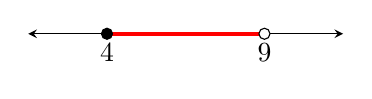
\begin{tikzpicture}[baseline=(current bounding box.north)]
    \coordinate (A) at (0,0);
    \coordinate (B) at (2,0);
    \draw [<->, >=stealth] (-1,0) -- (3,0);
    \node at (A) [anchor = north] {$4$};
    \node at (B) [anchor = north] {$9$};
    \draw [red, ultra thick] (A) -- (B);
    \draw [fill=black] (A) circle (2pt);
    \draw [fill=white] (B) circle (2pt);
\end{tikzpicture} 
\\
\hline $(4, \, 9]$ & $\lbrace x \mid 4 < x \leq 9 \rbrace$ & 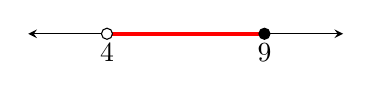
\begin{tikzpicture}[baseline=(current bounding box.north)]
    \coordinate (A) at (0,0);
    \coordinate (B) at (2,0);
    \draw [<->, >=stealth] (-1,0) -- (3,0);
    \node at (A) [anchor = north] {$4$};
    \node at (B) [anchor = north] {$9$};
    \draw [red, ultra thick] (A) -- (B);
    \draw [fill=white] (A) circle (2pt);
    \draw [fill=black] (B) circle (2pt);
\end{tikzpicture} 
\\[0.15in]  \hline
\end{tabular}}
\end{center}
\end{frame}


\begin{frame}{Interval Notation}
\begin{center}
\setlength{\extrarowheight}{8pt}
\scalebox{0.9}{
\begin{tabular}{|c|c|c|}
\hline \textbf{Interval Notation} & \textbf{Set-Builder Notation} & \textbf{Graph} \\[5pt] 
\hline $(4, \, \infty)$ & $\lbrace x \mid x > 4 \rbrace$ & 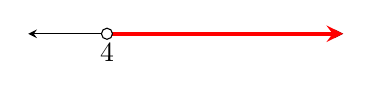
\begin{tikzpicture}[baseline=(current bounding box.north)]
    \coordinate (A) at (0,0);
    \coordinate (B) at (2,0);
    \draw [<->, >=stealth] (-1,0) -- (3,0);
    \node at (A) [anchor = north] {$4$};
    \draw [red, ultra thick, ->, >=stealth] (A) -- (3,0);
    \draw [fill=white] (A) circle (2pt);
\end{tikzpicture} 
\\

\hline $[4, \, \infty)$ & $\lbrace x \mid x \geq 4 \rbrace$ & 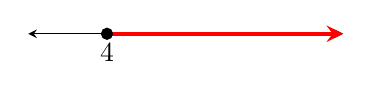
\begin{tikzpicture}[baseline=(current bounding box.north)]
    \coordinate (A) at (0,0);
    \coordinate (B) at (2,0);
    \draw [<->, >=stealth] (-1,0) -- (3,0);
    \node at (A) [anchor = north] {$4$};
    \draw [red, ultra thick, ->, >=stealth] (A) -- (3,0);
    \draw [fill=black] (A) circle (2pt);
\end{tikzpicture} 
\\

\hline $(-\infty, \, 9)$ & $\lbrace x \mid x < 9 \rbrace$ & 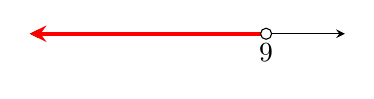
\begin{tikzpicture}[baseline=(current bounding box.north)]
    \coordinate (A) at (0,0);
    \coordinate (B) at (2,0);
    \draw [<->, >=stealth] (-1,0) -- (3,0);
    \node at (B) [anchor = north] {$9$};
    \draw [red, ultra thick, ->, >=stealth] (B) -- (-1,0);
    \draw [fill=white] (B) circle (2pt);
\end{tikzpicture} 
\\

\hline $(-\infty, \, 9]$ & $\lbrace x \mid x \leq 9 \rbrace$ & 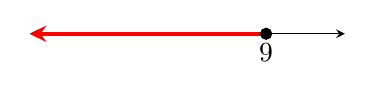
\begin{tikzpicture}[baseline=(current bounding box.north)]
    \coordinate (A) at (0,0);
    \coordinate (B) at (2,0);
    \draw [<->, >=stealth] (-1,0) -- (3,0);
    \node at (B) [anchor = north] {$9$};
    \draw [red, ultra thick, ->, >=stealth] (B) -- (-1,0);
    \draw [fill=black] (B) circle (2pt);
\end{tikzpicture} 
\\[0.15in]  \hline
\end{tabular}}
\end{center}
\end{frame}

\begin{frame}{Interval Notation}
\begin{center}
\setlength{\extrarowheight}{8pt}
\scalebox{0.9}{
\begin{tabular}{|c|c|c|}
\hline \textbf{Interval Notation} & \textbf{Set-Builder Notation} & \textbf{Graph} \\[5pt] 
\hline $(-\infty, \, \infty)$ & $\mathbb{R}$ & 

\begin{tikzpicture}[baseline=(current bounding box.north)]
    \draw [<->, >=stealth, red, ultra thick] (-1,0) -- (3,0);
\end{tikzpicture} 
\\[0.15in]

\hline  $\varnothing$   & $\{ \, \}$ & 
\begin{tikzpicture}[baseline=(current bounding box.north)]
    \draw [<->, >=stealth] (-1,0) -- (3,0);
\end{tikzpicture} 
\\[0.15in]  \hline
\end{tabular}} 
\end{center}
\end{frame}

\begin{frame}{Example 1}
Express each interval in set-builder notation and graph:    \newline\\
(a) \quad $(-1, \, 4]$  \newline\\

\onslide<2->{
\begin{center}
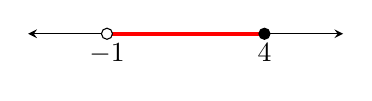
\begin{tikzpicture}[baseline=(current bounding box.north)]
    \coordinate (A) at (0,0);
    \coordinate (B) at (2,0);
    \draw [<->, >=stealth] (-1,0) -- (3,0);
    \node at (A) [anchor = north] {$-1$};
    \node at (B) [anchor = north] {$4$};
    \draw [red, ultra thick] (A) -- (B);
    \draw [fill=white] (A) circle (2pt);
    \draw [fill=black] (B) circle (2pt);
\end{tikzpicture} 
\end{center}
}

\onslide<3->{
\[  \{ x \mid -1 < x \leq 4 \}  \]
}
\end{frame}

\begin{frame}{Example 1}
(b) \quad $[2.5, \, 4]$ \newline\\

\onslide<2->{
\begin{center}
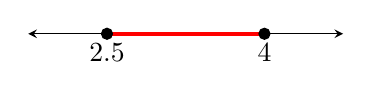
\begin{tikzpicture}[baseline=(current bounding box.north)]
    \coordinate (A) at (0,0);
    \coordinate (B) at (2,0);
    \draw [<->, >=stealth] (-1,0) -- (3,0);
    \node at (A) [anchor = north] {$2.5$};
    \node at (B) [anchor = north] {$4$};
    \draw [red, ultra thick] (A) -- (B);
    \draw [fill=black] (A) circle (2pt);
    \draw [fill=black] (B) circle (2pt);
\end{tikzpicture} 
\end{center}
}

\onslide<3->{
\[  \{ x \mid 2.5 \leq x \leq 4 \}   \]
}
\end{frame}


\begin{frame}{Example 1}
(c) \quad   $(-4, \, \infty)$   \newline\\

\onslide<2->{
\begin{center}
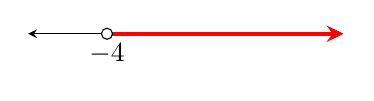
\begin{tikzpicture}[baseline=(current bounding box.north)]
    \coordinate (A) at (0,0);
    \coordinate (B) at (2,0);
    \draw [<->, >=stealth] (-1,0) -- (3,0);
    \node at (A) [anchor = north] {$-4$};
    \draw [red, ultra thick, ->, >=stealth] (A) -- (3,0);
    \draw [fill=white] (A) circle (2pt);
\end{tikzpicture} 
\end{center}
}

\onslide<3->{
\[  \{ x \mid x > -4 \} \]
}
\end{frame}

\begin{frame}{Example 1}
(d) \quad   $(-\infty, \, 5]$   \newline\\
\onslide<2->{
\begin{center}
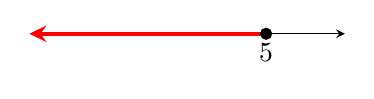
\begin{tikzpicture}[baseline=(current bounding box.north)]
    \coordinate (A) at (0,0);
    \coordinate (B) at (2,0);
    \draw [<->, >=stealth] (-1,0) -- (3,0);
    \node at (B) [anchor = north] {$5$};
    \draw [red, ultra thick, ->, >=stealth] (B) -- (-1,0);
    \draw [fill=black] (B) circle (2pt);
\end{tikzpicture}
\end{center}
}

\onslide<3->{
\[  \{ x \mid x \leq 5  \}  \]
}
\end{frame}

\section{Finding intersections and unions of intervals}

\begin{frame}{Intersections}
The \alert{intersection} of two sets is the set of elements that both sets have in common. \newline\\  \pause

The word \textsc{AND} is associated with intersections of sets.
\newline\\  \pause

The intersection of sets $A$ and $B$ is denoted
\[
    A \cap B
\]
\pause

Intersections are common when the variable is \emph{between} two values.
\end{frame}

\begin{frame}{Unions}
The \alert{union} of two sets is set of elements in either set (or both).   \newline\\  \pause 

The word \textsc{OR} is associated with the unions of sets.
\newline\\  \pause

The union of sets $A$ and $B$ is denoted
\[
    A \cup B
\]
\pause

Unions are common when the intervals do not overlap (although they can).
\end{frame}

\begin{frame}{Example 2}
Write each of the following in interval notation and graph. \newline\\
(a) \quad $x \leq 4 \text{ or } x > 7$  \newline\\
\onslide<2->{
\begin{center}
    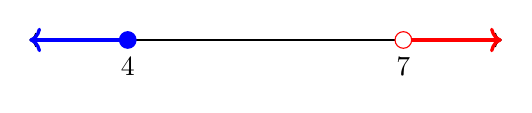
\begin{tikzpicture}
    \draw[<->] (-3,0) -- (3,0);
    \draw (-1.75,0.1) -- (-1.75,-0.1) node [below] {$4$};
    \draw (1.75,0.1) -- (1.75,-0.1) node [below] {$7$};
    \onslide<3->{\draw [->, very thick, color=blue] (-1.75,0) -- (-3,0);}
    \onslide<3->{\draw[color=blue,fill=blue] (-1.75,0) circle (3pt);}
    \onslide<4->{\draw[->, very thick, color=red] (1.75,0) -- (3,0);}
    \onslide<4->{\draw[color=red,fill=white] (1.75,0) circle (3pt);}
    \end{tikzpicture}
\end{center}
}

\onslide<5->{
\[  {\color{blue}(-\infty, 4]} \cup {\color{red}(7, \infty)}  \]
}
\end{frame}

\begin{frame}{Example 2}
(b) \quad $x < 2 \text{ or } x \geq 9$  \newline\\
\onslide<2->{
\begin{center}
    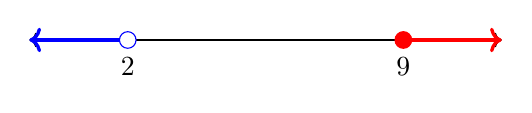
\begin{tikzpicture}
    \draw[<->] (-3,0) -- (3,0);
    \draw (-1.75,0.1) -- (-1.75,-0.1) node [below] {$2$};
    \draw (1.75,0.1) -- (1.75,-0.1) node [below] {$9$};
    \onslide<3->{\draw [->, very thick, color=blue] (-1.75,0) -- (-3,0);}
    \onslide<3->{\draw[color=blue,fill=white] (-1.75,0) circle (3pt);}
    \onslide<4->{\draw[->, very thick, color=red] (1.75,0) -- (3,0);}
    \onslide<4->{\draw[color=red,fill=red] (1.75,0) circle (3pt);}
    \end{tikzpicture}
\end{center}
}

\onslide<5->{
\[  {\color{blue}(-\infty, 2)} \cup {\color{red}[9, \infty)}  \]
}
\end{frame}


\begin{frame}{Example 2}
(c) \quad $0 < x \leq 5$  \newline\\
\onslide<2->{
\begin{center}
    \begin{tikzpicture}
    \draw[<->] (-3,0) -- (3,0);
    \draw (-1.75,0.1) -- (-1.75,-0.1) node [below] {$0$};
    \draw (1.75,0.1) -- (1.75,-0.1) node [below] {$5$};
    \onslide<3->{\draw [->, very thick, color=blue] (-1.75,1) -- (3,1);}
    \onslide<3->{\draw[color=blue,fill=white] (-1.75,1) circle (3pt);}
    \onslide<4->{\draw[->, very thick, color=red] (1.75,-1) -- (-3,-1);}
    \onslide<4->{\draw[color=red,fill=red] (1.75,-1) circle (3pt);}
    \onslide<5->{\draw[color=violet,ultra thick] (-1.75,0) -- (1.75,0);}
    \onslide<5->{\draw[color=violet,fill=white] (-1.75,0) circle (3pt);}
    \onslide<5->{\draw[color=violet,fill=violet] (1.75,0) circle (3pt);}
    \onslide<6->{\draw [color=white,fill=white] (-2,0.75) rectangle (3.5,1.25);}
    \onslide<6->{\draw [color=white,fill=white] (-3.25,-0.75) rectangle (3.25,-2);}
    \end{tikzpicture}
\end{center}
}

\onslide<6->{
\[  (0, \, 5]  \]
}
\end{frame}


\begin{frame}{Example 1}
(d) \quad $-5 \leq x \leq -3$   \newline\\
\onslide<2->{
\begin{center}
    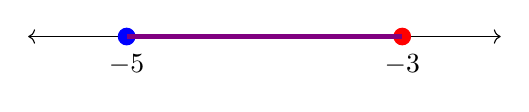
\begin{tikzpicture}
    \draw[<->] (-3,0) -- (3,0);
    \draw (-1.75,0.1) -- (-1.75,-0.1) node [below] {$-5$};
    \draw (1.75,0.1) -- (1.75,-0.1) node [below] {$-3$};
    \onslide<3->{\draw[color=blue,fill=blue] (-1.75,0) circle (3pt);}
    \onslide<4->{\draw[color=red,fill=red] (1.75,0) circle (3pt);}
    \onslide<5->{\draw [color=violet, ultra thick] (-1.75,0) -- (1.75,0);}
    \end{tikzpicture}
\end{center}
}

\onslide<6->{
\[  [-5, \, -3]  \]
}
\end{frame}

\begin{frame}{Example 3}
Write each of the following in interval notation and graph. \newline\\
(a) \quad $\{x \mid x \neq 0\}$ \newline\\
\onslide<2->{
\begin{center}
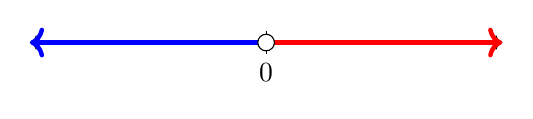
\begin{tikzpicture}
\draw[<->] (-3,0) -- (3,0);
\draw (0,0.15) -- (0,-0.15) node [below] {0};
\onslide<3->{
\draw[->, ultra thick, color=blue] (0,0) -- (-3,0);
\draw[->, ultra thick, color=red] (0,0) -- (3,0);
\draw[fill=white] (0,0) circle (3pt);}
\end{tikzpicture}
\end{center}
}

\onslide<4->{
\[
{\color{blue} (-\infty, 0)} \cup {\color{red}(0, \infty)}
\]
}
\end{frame}


\begin{frame}{Example 3}
Write each of the following in interval notation and graph. \newline\\
(b) \quad $\{x \mid x \neq 0, \, 2\}$ \newline\\
\onslide<2->{
\begin{center}
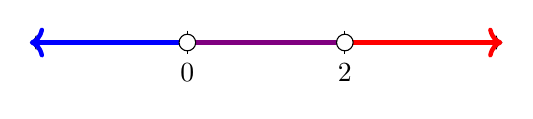
\begin{tikzpicture}
\draw[<->] (-3,0) -- (3,0);
\draw (-1,0.15) -- (-1,-0.15) node [below] {0};
\draw (1,0.15) -- (1,-0.15) node [below] {2};
\onslide<3->{
\draw[->, ultra thick, color=blue] (-1,0) -- (-3,0);
\draw[->, ultra thick, color=red] (1,0) -- (3,0);
\draw[color=violet, ultra thick] (-1,0) -- (1,0);
\draw[fill=white] (-1,0) circle (3pt);
\draw[fill=white] (1,0) circle (3pt);
}
\end{tikzpicture}
\end{center}
}

\onslide<4->{
\[
{\color{blue} (-\infty, 0)} \cup {\color{violet}(0,2)} \cup {\color{red}(2, \infty)}
\]
}
\end{frame}

\begin{frame}{Example 3}
Write each of the following in interval notation and graph. \newline\\
(c) \quad $\{x \mid x \neq -1, \, 1, \, 3\}$ \newline\\
\onslide<2->{
\begin{center}
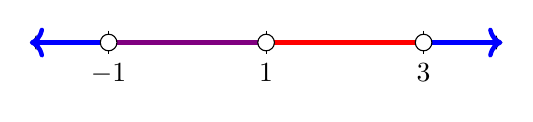
\begin{tikzpicture}
\draw[<->] (-3,0) -- (3,0);
\draw (-2,0.15) -- (-2,-0.15) node [below] {$-1$};
\draw (0,0.15) -- (0,-0.15) node [below] {1};
\draw (2,0.15) -- (2,-0.15) node [below] {3};
\onslide<3->{
\draw[->, ultra thick, color=blue] (-2,0) -- (-3,0);
\draw[->, ultra thick, color=blue] (2,0) -- (3,0);
\draw[color=violet, ultra thick] (-2,0) -- (0,0);
\draw[color=red, ultra thick] (0,0) -- (2,0);
\draw[fill=white] (-2,0) circle (3pt);
\draw[fill=white] (0,0) circle (3pt);
\draw[fill=white] (2,0) circle (3pt);
}
\end{tikzpicture}
\end{center}
}

\onslide<4->{
\[
{\color{blue} (-\infty, -1)} \cup {\color{violet}(-1,1)} \cup {\color{red}(1, 3)} \cup {\color{blue}(3, \infty)}
\]
}
\end{frame}

\end{document}


